\documentclass[12pt]{exam}
\usepackage[utf8]{inputenc}
\usepackage[T1]{fontenc}
\usepackage{wrapfig}
\usepackage{amsmath}
\usepackage{amssymb}
\usepackage{hyperref}
\usepackage{graphicx}
\usepackage[norsk]{babel}
\usepackage{tikz}
\usepackage{tkz-euclide}
\usepackage{float}
\usepackage{wrapfig}
\usepackage{pgfplots}
\pgfplotsset{compat=1.11}


\begin{document}

\pagestyle{headandfoot}
\runningheadrule
\firstpageheader{}{}{}
\firstpagefooter{}{}{}
\runningheader{Eksamenskurs i matematikk for ungdomskolen 2018}{}{\includegraphics[width=0.2\textwidth]{./img/logo.jpg}}
\runningfooter{}{}{}



{  \centering

	{\scshape\Huge Eksamenskurs i matematikk \par}
	\vspace{1cm}
	{\Large Ungdomskolen \today \par}
	\vspace{1.5cm}
        \begin{center}
          { \large
          \begin{tabular}{c | c}
            Tid & Hva \\ \hline
            16:15-17:30 & Del 1 : Linære funksjoner\\ \hline
            17:30-17:45 & Pause \\\hline
            17:45-19:00 & Del 2 : Linære likninger\\\hline
          \end{tabular}
          }
          \vspace{1.5cm}
          \begin{figure}[h!]
            \centering
            \includegraphics[scale = 0.7]{./img/forside.png}                      
          \end{figure}

        \end{center}

}

\newpage

\qformat{\underline{Spørsmål \thequestion} \hfill}
\section*{Linære funksjoner}
% Intro
\[
y = a\cdot x + b
\]
Vi kaller da:
\begin{itemize}
\item $a$ stigningstall
\item $b$ kontantledd
\item $x$ variabel
\end{itemize}
Vi oppgir punkter i $(x,y)$ koordinater.

% Oppgave 1
\begin{questions}
\question Sett punktene $(-1,4)-(-2,-5)-(3,1)-(4,9)-(2,-3)$ inn i koordinatsystemet.

\begin{center}

\begin{tikzpicture}[scale = 0.7,every node/.style={scale=0.6}]
\tkzInit[xmin=-10,xmax=10,ymin=-10,ymax=10]
\tkzGrid[color=gray]
\tkzAxeXY[very thick]
\end{tikzpicture}
\end{center}
\newpage
% Oppgave 2

\question På figuren ser du grafen til en funksjon.\\


\begin{minipage}[c]{0.5\textwidth}
\begin{parts}
\part Hva er stigningstallet?
\part Hva er konstantleddet?
\part Skriv opp likningen for linja.
\part Hva er nullpunktet?
\part Hva er $y$ når $x=1$?
\end{parts}
\end{minipage}%
\begin{minipage}[c]{0.45\textwidth}
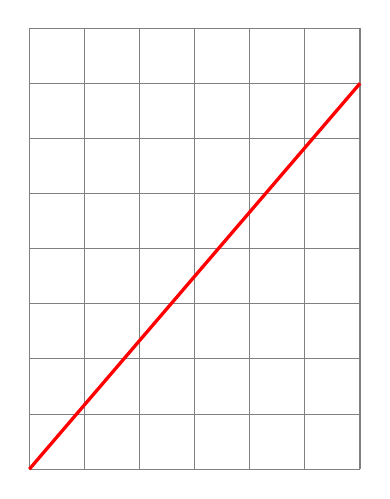
\begin{tikzpicture}[scale = 0.7,every node/.style={scale=0.6}]
\tkzInit[xmin=-1,xmax=5,ymin=-5,ymax=3]
\tkzGrid[color=gray]
\tkzAxeXY[very thick]
\draw[red,very thick] (-1,-5) -- (5,2);
\end{tikzpicture}  
\end{minipage}%\hfill


% Oppgave 3
\question 
\begin{parts}
\part 
\begin{minipage}{0.45\textwidth}
Fyll inn verditabell for $y=-x+5$
\end{minipage}
\begin{minipage}{0.5\textwidth}
{ \large
  \begin{tabular}{c | c | c|c}
    $x$ & -2 & 1 & 5 \\ \hline
    $y$ & \hspace{5mm} & \hspace{5mm} & \hspace{5mm}
  \end{tabular}
}
\end{minipage}

\part Tegn linja $-x+5$ i koordinatsystemet nedenfor  


\begin{tikzpicture}[scale = 1.1]
\tkzInit[xmin=-2,xmax=6,ymin=-2,ymax=6]
\tkzGrid[color=gray]
\tkzAxeXY[very thick]
\end{tikzpicture}  
\part En linje har konstantledd -2 og stigningstall 3. Tegn denne linja i koordinatsystemet ovenfor.
\end{parts}


% Oppgave 4
\question Hva er funksjonsuttrykket til linjene $f$, $g$, $h$ og  $i$ under (dvs hva er stigningstall og konstantledd?)

\begin{center}
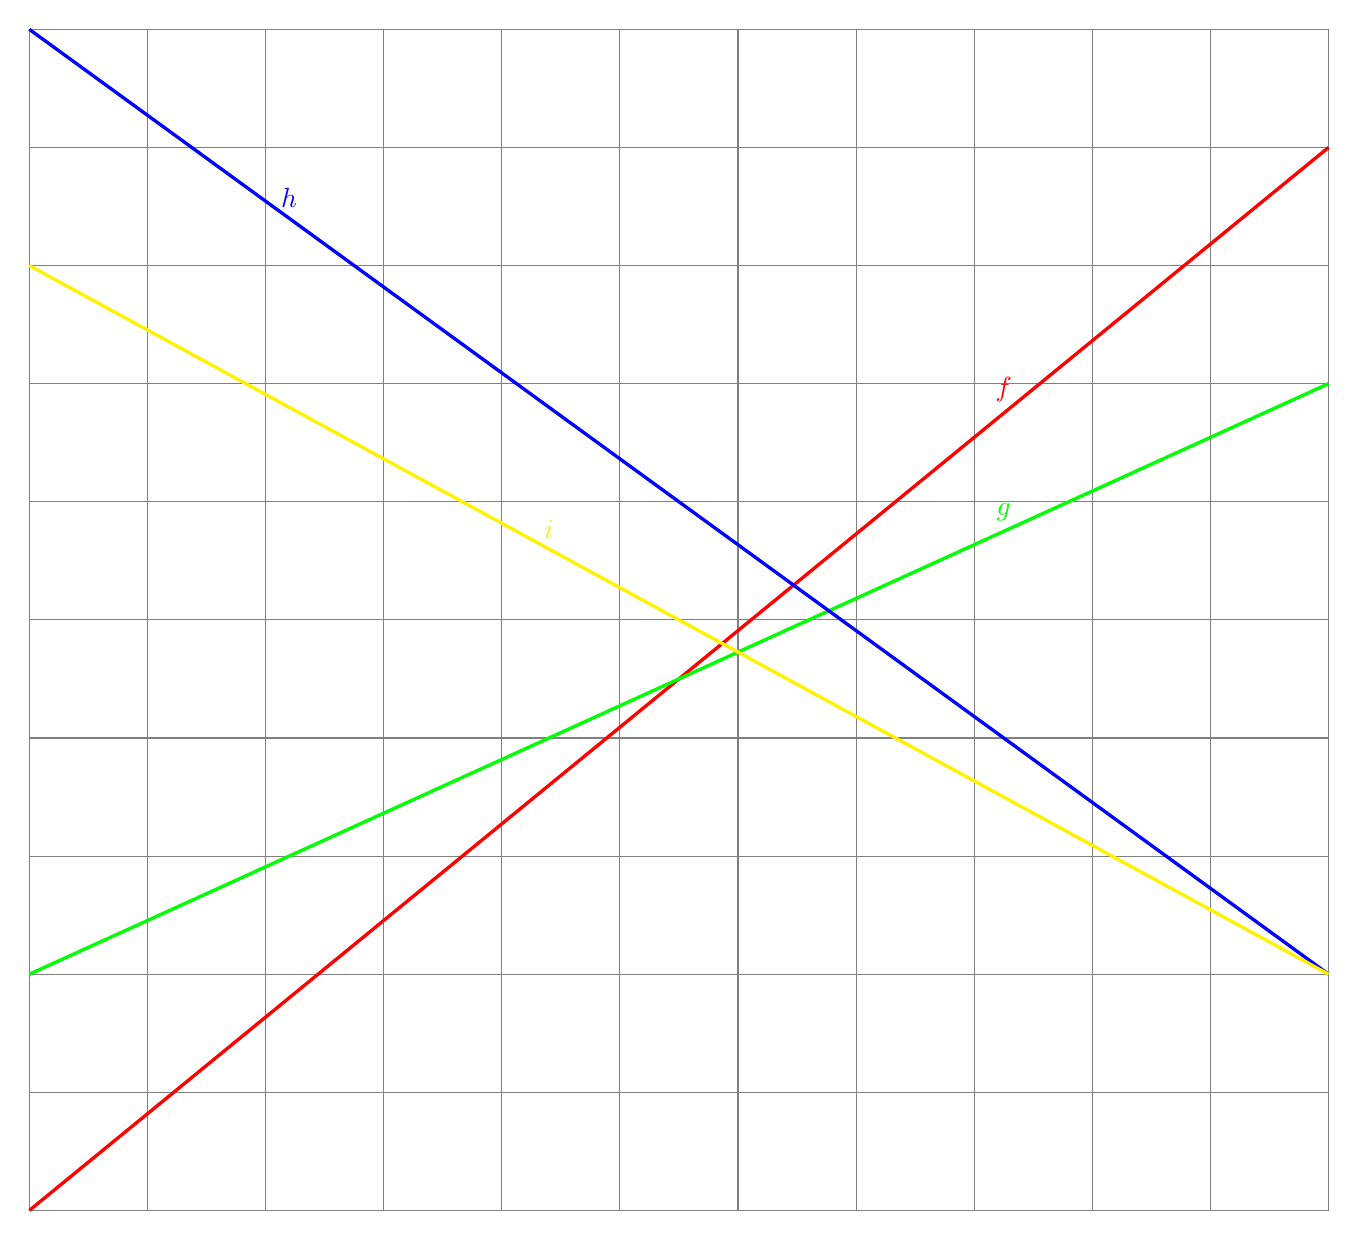
\begin{tikzpicture}[scale = 1.5,every node/.style={scale=1.0}]
\tkzInit[xmin=-6,xmax=5,ymin=-3,ymax=7]
\tkzGrid[color=gray]
\tkzAxeXY[very thick]
\draw[very thick, red] (-6,-3)   --   (5,6) node [near end,above] {$f$};
\draw[very thick, green] (-6,-1) --   (5,4) node [near end,above] {$g$};
\draw[very thick, blue] (-6,7)   --   (5,-1) node [pos=0.2,above] {$h$};
\draw[very thick, yellow] (-6,5) --   (5,-1) node [pos=0.4,above] {$i$};
\end{tikzpicture}  
\end{center}


\newpage
% Oppgave 5
\question Proposjonale funksjoner.
Kjennetegnes ved at den lineære funksjonen går gjennom origo. Den mangler derfor konstantleddet (eller du kan si at  konstantleddet er null) og skrive derfor på formen $y = a \cdot x$.

{\it Proporsjonalt} – vil si at verdien til funksjonen langs $x$-aksen vokser proporsjonalt med verdien langs $y$-aksen (''i samme takt''). Forholdet mellom $y$ og $x$ blir stigningstallet men kalles oftest $k$ proporsjonalitetskonstanten.

\[
y  = kx \to \frac{y}{x} = k
\]

\begin{parts}
\part Hvilke av disse funksjonene er proposjonale?
\begin{choices}
\choice 
$y = 2x + 3$
\choice 
$y = x + 5$
\choice
$y = -x + -2$
\choice
$y = -4x + -6$
\end{choices}

\part Er antall Gb data inkludert i abonnementet proporsjonal med prisen du betaler i følge denne tabellen?\\
\begin{center}
\begin{tabular}[h!]{c|c|c|c|c}
{\bf Navn abonnement} & {\bf Frosk}  & {\bf Padde}  & {\bf Alligator}  & {\bf Streptosaurus} \\ \hline
{\bf Antall Gb.} & 2 & 5 & 12 & 20 \\ \hline  
{\bf Pris pr. måned} & 120 & 300 & 480 & 900 \\ 
\end{tabular}
\end{center}

\part En bonde selger poteter i store sekker på 10kg, 50 kg, eller 120 kg.  Bestem de manglende prisene i tabellen for at forholdet mellom kg og pris skal være proporsjonalt. 
{ \large
\begin{center}
\begin{tabular}[h!]{c|c|c|c|c}
{\bf Antall kg i sekken} & 10 & 50 & 120 & 250 \\ \hline  
{\bf Pris pr. sekk} & $$ & 150 & $$ & $$ \\ \hline  
\end{tabular}
\end{center}
}

\part Figuren viser hvordan lønna til Svein varierer med antall timer han jobber.\\

\begin{center}
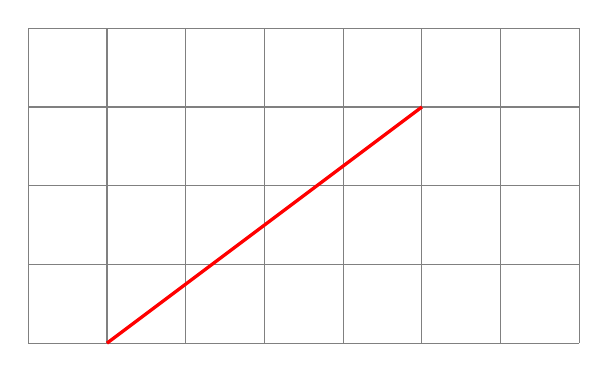
\begin{tikzpicture}[scale = 1.0]
\tkzInit[xmin=-1,xmax=6,ymin=0,ymax=800, ystep = 200]
\tkzGrid[color=gray]
\tkzAxeXY[very thick]
\draw[very thick, red] (0,0) -- (4,3);
\end{tikzpicture}  
\end{center}

\begin{choices}
\choice Hvor mye tjener Svein i timen?
\choice I løpet av en uke jobbet Svein i 15 timer. Hvor mye tjente han den uka?
\end{choices}

\end{parts}

\end{questions}


\end{document}





